\documentclass[aspectratio=169]{beamer}

\usetheme{metropolis}
\usepackage[utf8]{inputenc}
\usepackage{graphicx}
\usepackage{booktabs}
\usepackage{graphicx}
\usepackage[dvipsnames]{xcolor}
\usepackage[backend=biber,style=numeric,sorting=none]{biblatex}
\usepackage{csquotes}
\usepackage[spanish]{babel}
\usepackage{ragged2e}
\usepackage{setspace}
\usepackage{bookmark}
\usepackage[version=4]{mhchem}
\usepackage{microtype}
\usepackage{booktabs}
\usepackage{hyperref}

\addbibresource{TEM.bib}

\title{Microscopía Electrónica de Transmisión (TEM)}
\subtitle{Técnica de Caracterización de Nanomateriales}
\date{\today}
\author{Acuña-Avila-Huertas-Martínez-Parada-Rodriguez}


\begin{document}

\maketitle

\begin{frame}{Contenido}
  \setbeamertemplate{section in toc}[sections numbered]
  \tableofcontents
\end{frame}

\section{Contexto Histórico}

\begin{frame}{Contexto Histórico - La barrera clásica (1873)}
\textbf{Ernst Abbe} demostró que la resolución depende de la difracción, no solo de la calidad de las lentes.

\vspace{0.6em}
\[
  d = \frac{\lambda}{2n\sin\alpha} = \frac{\lambda}{2NA}
\]

\begin{itemize}
  \item Para luz visible, el límite práctico es \(\sim 200\,\text{nm}\).
  \item Virus, proteínas y ultraestructura celular quedan fuera del alcance óptico.
  \item Abbe anticipó la salida: usar radiación con \(\lambda\) mucho menor.
\end{itemize}
\end{frame}

\begin{frame}{Contexto Historico - Antecedentes}
\begin{columns}[T,totalwidth=\textwidth]
\column{0.49\textwidth}
\textbf{Comportamiento ondulatorio de la materia}

\vspace{0.4em}
De Broglie (1924):
\[
\lambda = \frac{h}{p}
\]

Para electrones acelerados por un potencial \(V\):
\[
\lambda \approx \frac{h}{\sqrt{2m_e eV}}
\]

\begin{itemize}
  \item A \(100\,\text{kV}\), \(\lambda_e \approx 0.0037\,\text{nm}\).
  \item \(\lambda_e\) es más de \(10^5\) veces menor que la luz visible.
\end{itemize}

\column{0.49\textwidth}
\textbf{Trabajo de Hans Busch (1926)}

\vspace{0.4em}
Busch propuso que los \textbf{campos magnéticos} podían dirigir haces de electrones de forma análoga a las lentes ópticas.

\begin{itemize}
  \item Demostró que un haz de pequeño ángulo puede enfocarse en un punto con una lente magnética cilíndrica.
  \item Esta prueba fundó la óptica electrónica práctica.
  \item Fue la base directa del desarrollo del TEM.
\end{itemize}
\end{columns}
\end{frame}

\begin{frame}{Contexto Histórico - Nacimiento del TEM (1931--1933)}





En Berlín, \textbf{Max Knoll} y \textbf{Ernst Ruska} materializaron la óptica electrónica.

\begin{itemize}
  \item Base teórica: Hans Busch (1926), lentes magnéticas axials.
  \item 1931: primer prototipo funcional de microscopio electrónico.
  \item 1933: versión que supera la resolución de la microscopía óptica.
\end{itemize}

\vspace{0.6em}
\textbf{Controversia de patente:}
\begin{itemize}
  \item Siemens registró patente en 1931 antes de la presentación pública.
  \item El reconocimiento científico recayó en Ruska.
  \item Nobel de Física en 1986 por su contribución decisiva.
\end{itemize}
\end{frame}

\begin{frame}{Contexto Histórico - Impacto}
\begin{columns}[c,totalwidth=\textwidth]
\column{0.53\textwidth}
\textbf{Impacto científico}
\begin{itemize}
  \item Descubrimiento de ribosomas (Palade, 1955).
  \item Cartografía de retículo endoplásmico, Golgi, lisosomas y mitocondrias.
  \item Nobel de 1974 (Claude, Palade y de Duve).
\end{itemize}

\column{0.46\textwidth}
\begin{figure}
  \centering
  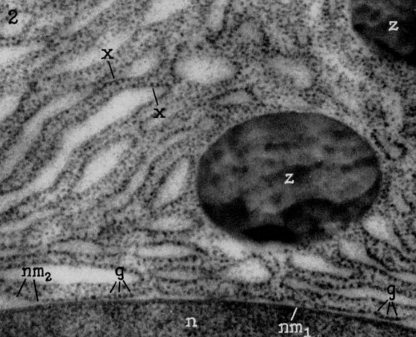
\includegraphics[width=\linewidth]{Screenshot_20260317_232844.png}
  \caption{Micrografía electrónica del retículo endoplásmico de células acinares pancreáticas de rata.}
\end{figure}
\end{columns}
\end{frame}

\section{Principios Físicos}
% SLIDE 1: Scattering
\begin{frame}{Formación de la Imagen: Dispersión y Atenuación}
    \begin{itemize}
        \item La base de la formación de la imagen es la dispersión del haz de electrones y su posterior interferencia.
        \item Las muestras deben ser ultradelgadas para reducir la atenuación de la señal.
    \end{itemize}
    \vspace{0.5cm}
    \textbf{Regímenes de Dispersión:}
    \begin{itemize}
        \item \textbf{Señal (Elástica):} Conservación de la energía. Interacciones núcleo-electrón (alto ángulo) y nube electrónica (bajo ángulo).
        \item \textbf{Ruido (Inelástica):} Transferencia de energía a la muestra. Generación de fonones, plasmones y radiación Bremsstrahlung.
    \end{itemize}
\end{frame}

% SLIDE 2: Coherence
\begin{frame}{El Requisito de Coherencia}
    Para formar una imagen mediante interferencia y mitigar el ruido inelástico, requerimos un haz altamente coherente.
    
    \vspace{0.5cm}
    \textbf{Componentes de la Coherencia:}
    \begin{itemize}
        \item \textbf{Coherencia Espacial (Transversal):} Depende del tamaño de la fuente. Requerimos una fuente que se aproxime a un punto ideal.
        \item \textbf{Coherencia Temporal (Longitudinal):} Depende de la dispersión de energía ($\Delta E$). Vital para evitar aberraciones cromáticas exacerbadas por la dispersión inelástica.
    \end{itemize}
\end{frame}

% SLIDE 3: Electron Guns
\begin{frame}{Generación del Haz: Termiónica vs. Emisión de Campo}
    \textbf{1. Emisión Termiónica}
    \begin{itemize}
        \item \textit{Física:} Requiere altas temperaturas (degrada el material) y produce una amplia distribución de velocidades (Maxwell-Boltzmann).
        \item \textit{Modelo (Richardson-Laue-Dushman)}:
        \begin{equation*}
            J = A_G T^2 \exp{(- \Phi T^{-1})}
        \end{equation*}
    \end{itemize}
\end{frame}
\begin{frame}
    \centering
    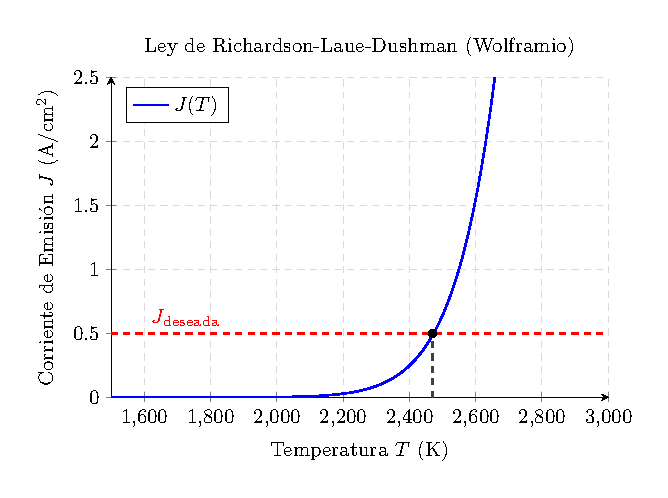
\includegraphics{emmision-current.pdf}
\end{frame}
\begin{frame}
    \textbf{2. Emisión de Campo Frío (CFEG) y Schottky}
    \begin{itemize}
        \item \textit{Física:} Un campo eléctrico deforma el potencial en una barrera triangular, permitiendo el efecto túnel cuántico.
        \item \textit{Ventaja:} Ancho de banda de energía muy estrecho ($\approx 0.3 \text{ eV}$), garantizando coherencia.
        \item \textit{Modelo (Fowler-Nordheim)}:
        \begin{equation*}
            J = A E^2 \Phi^{-1} \exp{\left(- B \Phi^{\frac{3}{2}}E^{-1}\right)}
        \end{equation*}
    \end{itemize}
\end{frame}

\section{El Instrumento (TEM)}
\begin{frame}{El Instrumento}
    \begin{itemize}
        \item El TEM opera bajo principios ópticos análogos a un microscopio óptico, pero utilizando electrones y campos electromagnéticos.
        \item La columna del microscopio se divide en tres sistemas fundamentales:
        \begin{enumerate}
            \item \textbf{Sistema de iluminación:} Cañón de electrones y lentes condensadoras.
            \item \textbf{Sistema formador de imagen:} Lente objetivo, portamuestras y aperturas.
            \item \textbf{Sistema de proyección y detección:} Lentes intermedias/proyectoras y detectores (cámaras CCD/CMOS).
        \end{enumerate}
        \item Todo el sistema requiere condiciones de ultra alto vacío ($10^{-7}$ a $10^{-9} \, \text{Torr}$) para evitar la dispersión del haz por moléculas de gas.
    \end{itemize}
\end{frame}
\begin{frame}
    \begin{center}
        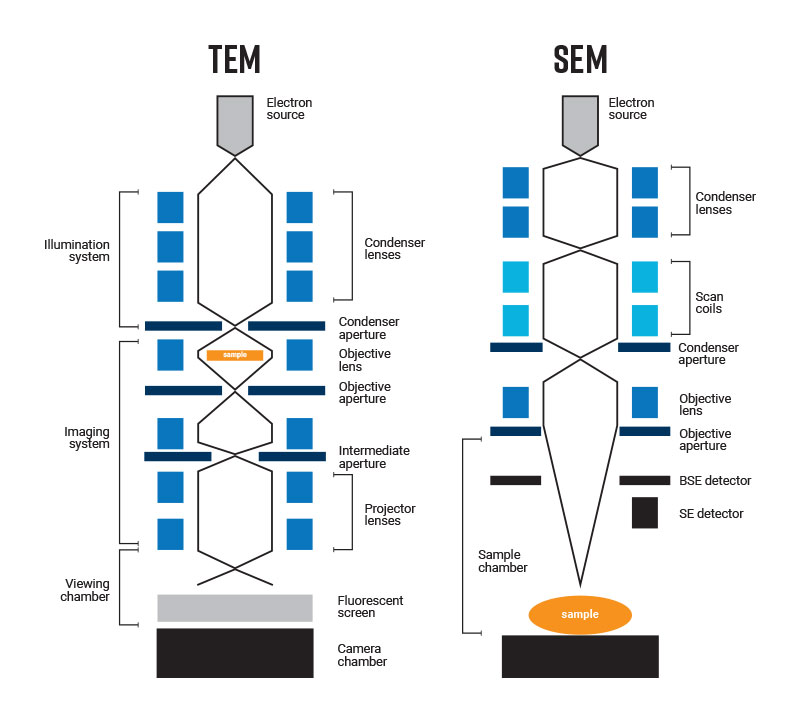
\includegraphics[width=0.5\textwidth]{images/SEMvTEM-Beam-Comparison-Figure.jpg} \\
        {\tiny Imagen obtenida de: \url{https://www.nanoscience.com/blogs/whats-the-difference-between-sem-and-tem/}}
    \end{center}
\end{frame}

\begin{frame}{Sistema de Iluminación: El Cañón de Electrones}
    \textbf{Generación del haz:}\\
        El cañón de electrones genera, acelera y enfoca el haz inicial. Típicamente operan a voltajes de aceleración entre $100\text{ keV}$ y $300\text{ keV}$.
    \vspace{0.2cm}
    Existen dos tecnologías principales:
    \begin{itemize}
        \item \textbf{Emisión Termoiónica:} Filamentos de Wolframio (W) o Hexaboruro de Lantano ($\text{LaB}_6$). Los electrones superan la función de trabajo del material mediante calentamiento.
        \item \textbf{Emisión de Campo (FEG):} Emplea un cristal de Wolframio muy afilado sometido a un intenso campo eléctrico. Ofrece mayor coherencia espacial, mayor brillo y una menor dispersión energética.
    \end{itemize}
\end{frame}

\begin{frame}{Lentes Electromagnéticas}
    \begin{columns}
        \begin{column}{0.5\textwidth}
            \begin{itemize}
                \item A diferencia de las lentes de vidrio, el TEM usa bobinas de alambre rodeadas por polos de hierro magnético.
                \item La trayectoria de los electrones se curva debido a la fuerza de Lorentz:
                $$ \mathbf{F} = -e(\mathbf{v} \times \mathbf{B}) $$
                \item Variando la corriente en las bobinas, se altera el campo magnético $\mathbf{B}$ y, por ende, la distancia focal de la lente.
            \end{itemize}
        \end{column}
        \begin{column}{0.5\textwidth}
            \begin{center}
                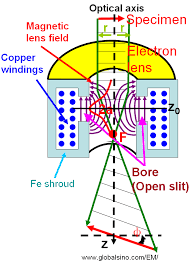
\includegraphics[width=0.4\textwidth]{images/lente_electromagnetica.png} \\
                {\tiny Imagen obtenida de: \url{http://www.cientificosaficionados.com/foros/viewtopic.php?t=17475}}
            \end{center}
        \end{column}
    \end{columns}
\end{frame}

\begin{frame}{Jerarquía de Lentes y Aperturas}
\begin{columns}
    \begin{column}{0.6\textwidth}
        \begin{itemize}
            \item \textbf{Lentes Condensadoras:} Controlan el tamaño del spot y la convergencia del haz que incide sobre la muestra.
            \item \textbf{Lente Objetivo:} Es el corazón del TEM. Determina el límite de resolución espacial. Las aberraciones esféricas ($C_s$) y cromáticas ($C_c$) son los principales factores limitantes.
            \item \textbf{Apertura de la Lente Objetivo:} Bloquea electrones dispersados a ángulos altos, mejorando significativamente el contraste de la imagen.   
        \end{itemize}
    \end{column}
    \begin{column}{0.4\textwidth}
        \begin{center}
            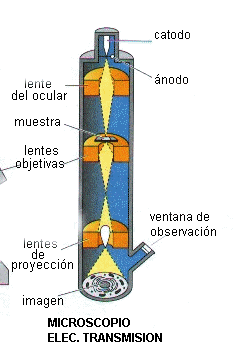
\includegraphics[width=0.5\textwidth]{images/microsc.png} \\
            {\tiny Imagen obtenida de: \url{https://www.biologia.edu.ar/microscopia/microscopia1.htm}}
        \end{center}
    \end{column}
\end{columns}
\end{frame}

\begin{frame}{Cámara de Muestra y Goniómetro}
\begin{columns}
        \begin{column}{0.6\textwidth}
            La muestra debe ser extremadamente delgada (típicamente $< 100\text{
            nm}$) para ser ``transparente'' a los electrones.
            \begin{itemize}
                \item \textbf{Portamuestras:} Varilla de precisión mecánica que inserta la rejilla de cobre o carbono en el centro del campo magnético de la lente objetivo.
                \item \textbf{Goniómetro:} Mecanismo que permite rotar e inclinar la muestra en los ejes $x$ e $y$ (tilt/double tilt) con precisión nanométrica.
                \item Vital para alinear ejes zonales cristalográficos paralelos al haz de electrones.
            \end{itemize}
        \end{column}
        \begin{column}{0.4\textwidth}
            \begin{center}
            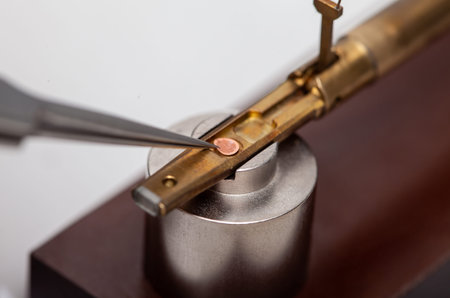
\includegraphics[width=0.8\textwidth]{images/portamuestras.jpg} \\
            {\tiny Imagen obtenida de: \url{https://es.123rf.com/photo_190998080_el-portamuestras-del-microscopio-electrónico-de-transmisión-se-ha-cargado-con-una-muestra-en-una-rej.html}}
    \end{center}
        \end{column}
    \end{columns}
\end{frame}

\begin{frame}{Detectores y Adquisición de Datos}
\begin{columns}
    \begin{column}{0.6\textwidth}
        Una vez que los electrones atraviesan la muestra y son magnificados por las lentes intermedias y proyectoras, inciden sobre el sistema de detección:
        \begin{itemize}
            \item \textbf{Pantalla fluorescente:} Para la visualización directa y alineación manual.
            \item \textbf{Cámaras Digitales (CCD/CMOS):} Convertidores de electrones en fotones y luego en señales digitales.
            \item \textbf{Cámaras de Detección Directa:} Sensores modernos que detectan los electrones incidentes sin conversión previa a luz, mejorando la relación señal/ruido (DQE).
        \end{itemize}
    \end{column}
    \begin{column}{0.4\textwidth}
        \begin{center}
            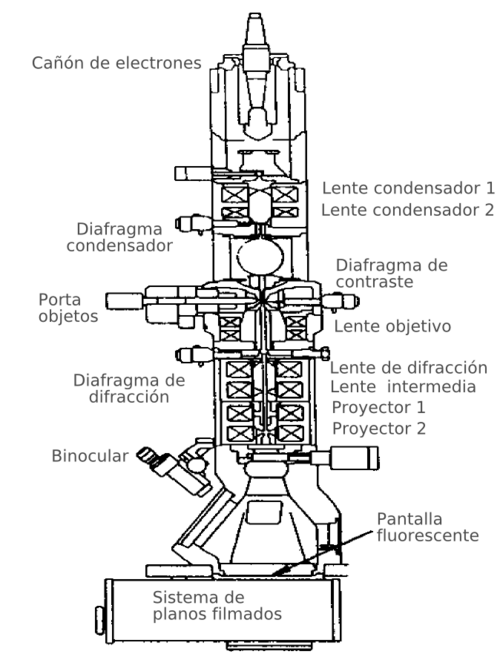
\includegraphics[width=0.5\textwidth]{images/scheme_TEM.png} \\
            {\tiny Imagen obtenida de:\url{https://es.wikipedia.org/wiki/Microscopio_electrónico_de_transmisión}}
        \end{center}
    \end{column}
\end{columns}    
\end{frame}

\section{Análisis de Imagen}
\begin{frame}{Análisis de Imágenes}
    \begin{itemize}
        \item \textbf{Campo Claro (Bright Field):} Zonas más densas o gruesas dispersan más electrones y se ven oscuras; el fondo vacío se ve brillante.
        
        \item \textbf{Difracción (SAED):} Permite analizar la estructura cristalográfica, diferenciando si el material es amorfo, policristalino o monocristalino.
        \item \textbf{Alta Resolución (HRTEM):} Utiliza contraste de fase para visualizar directamente los planos atómicos.
    \end{itemize}
\end{frame}

\begin{frame}{Imagen de campo claro}
\begin{itemize}
        \item Modo mas comun de operacion
        \item e transmitidos forman la img de campo claro
        \item Secciones oscuras (Mayor grosor, densidad, numero atomico)
        \item Proyeccion 2D de sample
    \end{itemize}
\end{frame}
\begin{frame}{Imagen de campo claro}
\begin{figure}
    \centering
    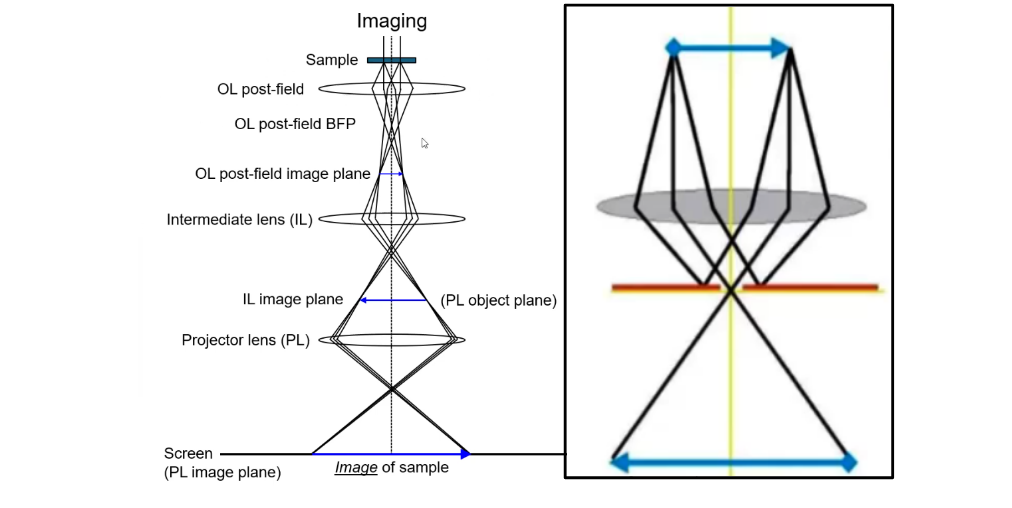
\includegraphics[width=1\linewidth]{0.png}
    \label{fig:placeholder}
\end{figure}
\end{frame}

\begin{frame}{Imagen de campo claro}
\begin{figure}
    \centering
    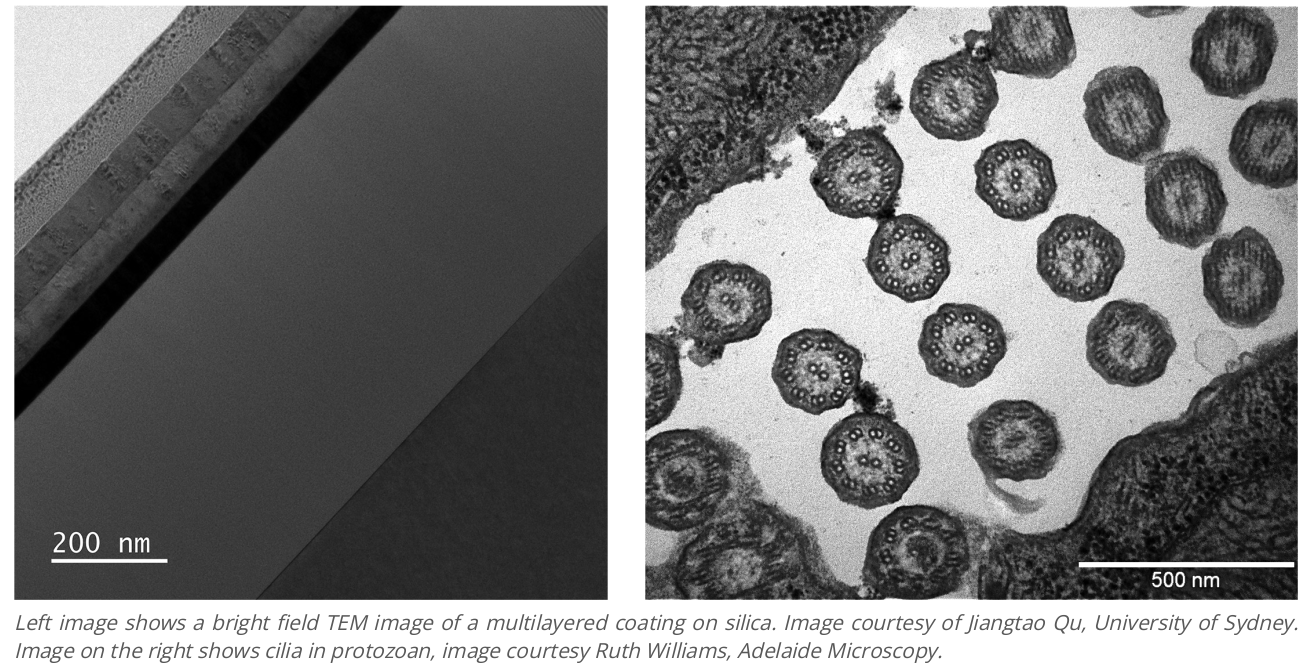
\includegraphics[width=1\linewidth]{image1.png}
    \label{fig:placeholder}
\end{figure}
\end{frame}

\begin{frame}{Imagen de campo oscuro}
\begin{itemize}

        \item e difractados forman la img de campo oscuro
        \item Permite identificar distintas prop no visibles en imagen de campo claro
        \item Aisla defectos o fases cristalinas
        
    \end{itemize}
\end{frame}
\begin{frame}{Imagen de campo oscuro}

\begin{figure}
    \centering
    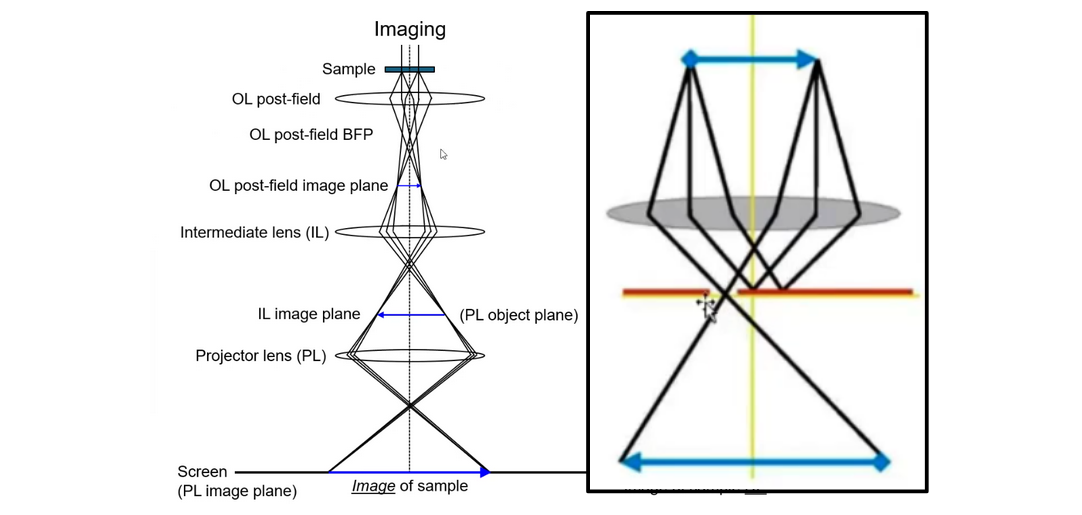
\includegraphics[width=1\linewidth]{3.png}
    \label{fig:placeholder}
\end{figure}

\end{frame}

\begin{frame}{Imagen de campo oscuro}
\begin{figure}
    \centering
    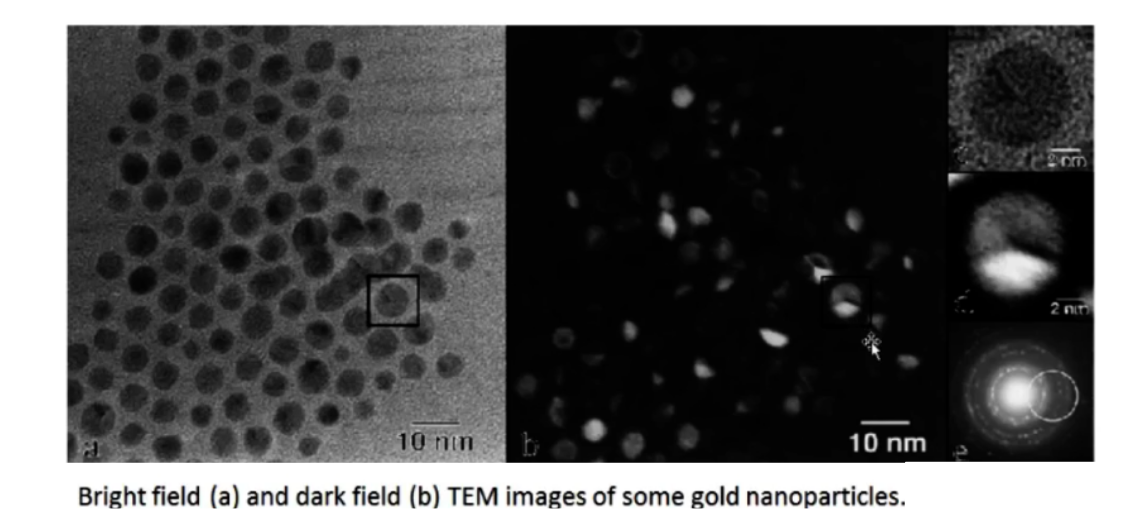
\includegraphics[width=1\linewidth]{2.png}
    \label{fig:placeholder}
\end{figure}
\end{frame}















\begin{frame}{Difraccion SAED}
\begin{itemize}

        \item ``Selected Area Electron Diffraction''
        \item Lente objetivo forma un patron de difraccion en el plano focal trasero
        \item Mediado por la potencia del lente intermedio
        \item Permite analizar la estructura cristalografica, diferenciando si el material es amorfo, policristalino o monocristalino.
        
    \end{itemize}
\end{frame}

\begin{frame}{Difraccion SAED}


\begin{figure}
    \centering
    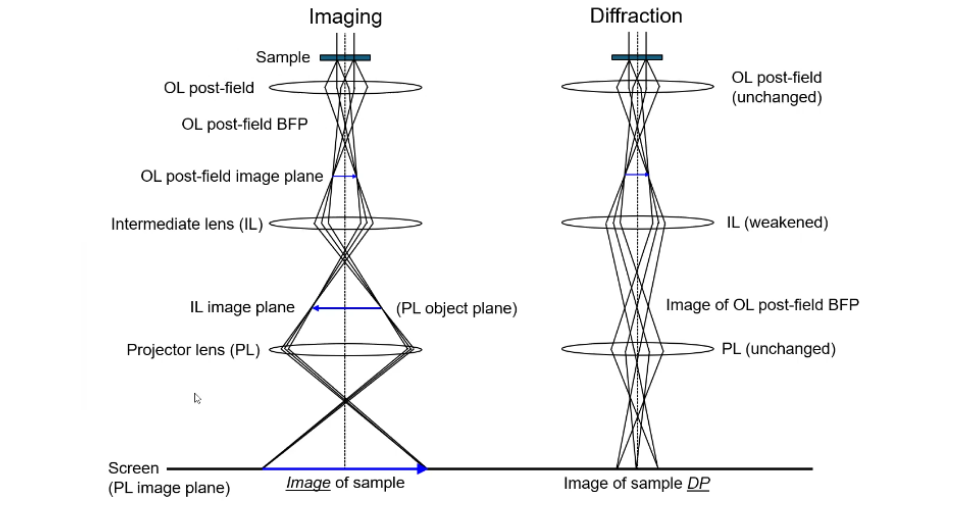
\includegraphics[width=1\linewidth]{5.png}
    \label{fig:placeholder}
\end{figure}

\end{frame}

\begin{frame}{Difraccion SAED}
\begin{figure}
    \centering
    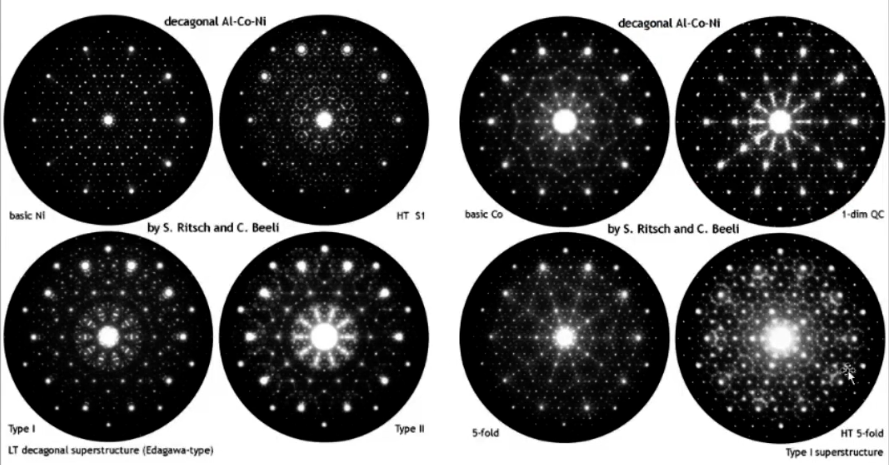
\includegraphics[width=1\linewidth]{6.png}
    \label{fig:placeholder}
\end{figure}
\end{frame}













\begin{frame}{Alta resolucion HRTEM}
\begin{itemize}

        \item visualizacion de la estructura atómica
        \item Utiliza constraste de fase utilizando los haces directos y difractados
        \item Al igual que en campo oscuro se pueden seleccionar ciertos rayos difractados
        
    \end{itemize}
\end{frame}

\begin{frame}{Alta resolucion HRTEM}


\begin{figure}
\begin{figure}
    \centering
    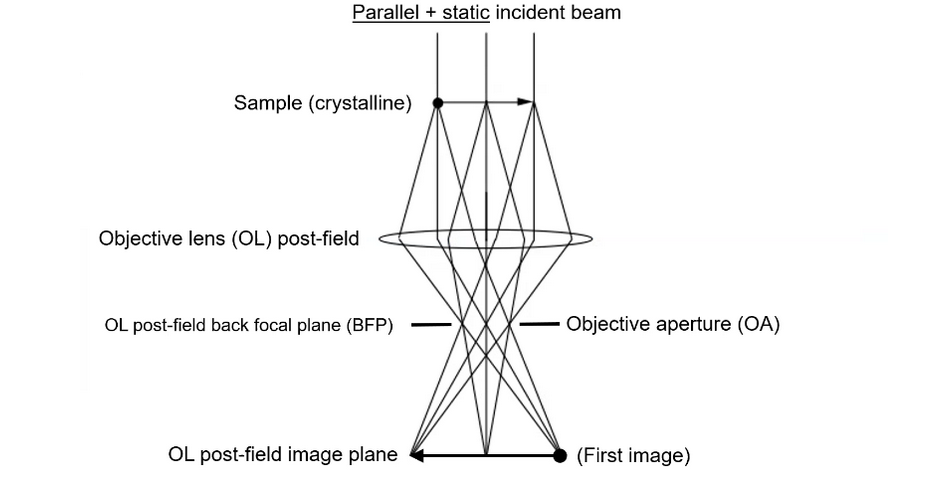
\includegraphics[width=1\linewidth]{8.png}
    \caption{Enter Caption}
    \label{fig:placeholder}
\end{figure}
\end{figure}

\end{frame}

\begin{frame}{Alta resolucion HRTEM}
\begin{figure}
    \centering
    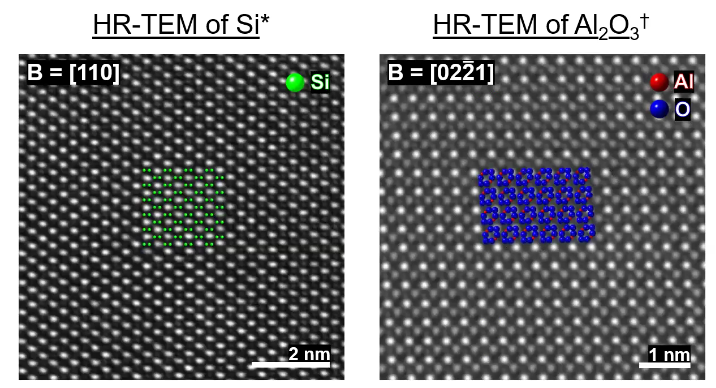
\includegraphics[width=1\linewidth]{7.png}
    \label{fig:placeholder}
\end{figure}
\end{frame}

\section{Ejemplo practico}
% Diapositiva 1: Nanotubos y Grafeno
\begin{frame}{1. Nanotubos de Carbono (CNTs) y Grafeno}
    \begin{columns}
        \begin{column}{0.55\textwidth}
            \textbf{Importancia y Aplicaciones:}
            \begin{itemize}
                \item Propiedades eléctricas, térmicas y mecánicas excepcionales.
                \item Uso en nanoelectrónica y almacenamiento de energía.
            \end{itemize}
            \vspace{0.3cm}
            \textbf{¿Por qué usar TEM?}
            \begin{itemize}
                \item Permite contar las paredes de grafeno (clasificar en SWCNT o MWCNT).
                \item Indispensable para observar defectos topológicos en la red hexagonal.
            \end{itemize}
        \end{column}
        \begin{column}{0.45\textwidth}
            \begin{figure}
                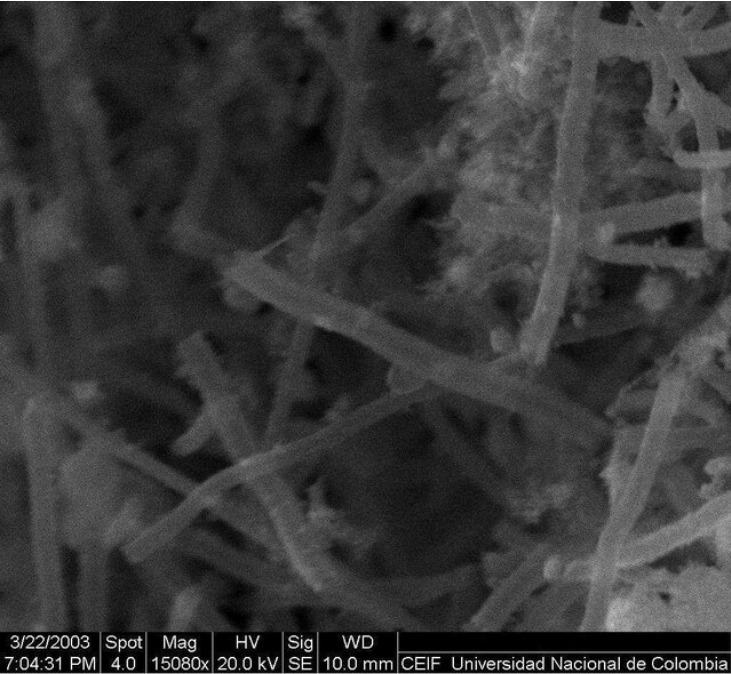
\includegraphics[width=\textwidth]{nano-tubos.png}
                \caption{\scriptsize Imagen TEM de nanotubos \cite{gallego2014hydrogen}.}
            \end{figure}
        \end{column}
    \end{columns}
\end{frame}

% Diapositiva 2: Nanopartículas Metálicas
\begin{frame}{2. Nanopartículas Metálicas}
    \begin{columns}
        \begin{column}{0.55\textwidth}
            \textbf{Importancia y Aplicaciones:}
            \begin{itemize}
                \item Destacan por la resonancia de plasmones superficiales.
                \item Uso en biosensores y catálisis.
            \end{itemize}
            \vspace{0.3cm}
            \textbf{¿Por qué usar TEM?}
            \begin{itemize}
                \item Revela la morfología exacta.
                \item En alta resolución (HRTEM), permite ver los planos cristalográficos.
            \end{itemize}
        \end{column}
        \begin{column}{0.45\textwidth}
            \begin{figure}
                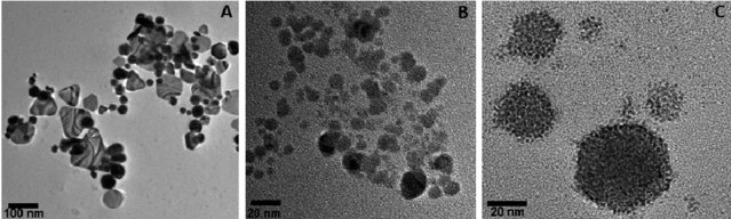
\includegraphics[width=\textwidth]{nano-oro.png}
                \caption{\scriptsize Nanopartículas de oro (A), plata (B) y platino (C), biosintetizadas con extractos de \textit{Neurospora crassa} \cite{castro2016centro}.}
            \end{figure}
        \end{column}
    \end{columns}
\end{frame}

% Diapositiva 3: Puntos Cuánticos
\begin{frame}{3. Puntos Cuánticos (Quantum Dots)}
    \begin{columns}
        \begin{column}{0.55\textwidth}
            \textbf{Ejemplos Específicos:}
            \begin{itemize}
                \item Puntos Cuánticos de Carbono (C-QDs).
                \item Semiconductores: Seleniuro de Cadmio (CdSe) o Sulfuro de Plomo (PbS).
            \end{itemize}
            \vspace{0.3cm}
            \textbf{¿Por qué usar TEM?}
            \begin{itemize}
                \item El tamaño dicta el color de emisión de luz; el TEM mide el diámetro con precisión atómica para asegurar uniformidad en los lotes.
            \end{itemize}
        \end{column}
        \begin{column}{0.45\textwidth}
            \begin{figure}
                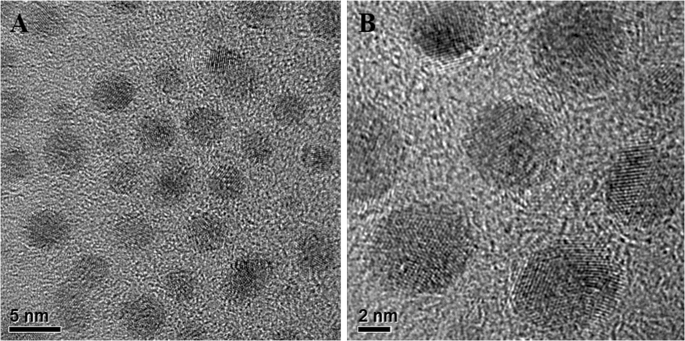
\includegraphics[width=\textwidth]{Qdots.png}
                \caption{\scriptsize C-QDs recién sintetizados. (A) Baja resolución, (B) Alta resolución, se aprecian las redes cristalinas \cite{dager2019synthesis}.}
            \end{figure}
        \end{column}
    \end{columns}
\end{frame}

% Diapositiva 4: Nanopartículas Core-Shell
\begin{frame}{4. Nanopartículas Core-Shell (Núcleo-Corteza)}
    \begin{columns}
        \begin{column}{0.5\textwidth}
            \textbf{Ejemplos Específicos:}
            \begin{itemize}
                \item NaYF$_4$:Yb/Tm@Au (Núcleo de tierras raras, corteza de oro).
                \item NaYF$_4$:Yb/Er@CdSe.
            \end{itemize}
            \vspace{0.3cm}
            \textbf{¿Por qué usar TEM?}
            \begin{itemize}
                \item Confirma la envoltura uniforme y mide su grosor. 
                \item El contraste por número atómico diferencia el núcleo de la corteza.
            \end{itemize}
        \end{column}
        \begin{column}{0.5\textwidth}
            \begin{figure}
                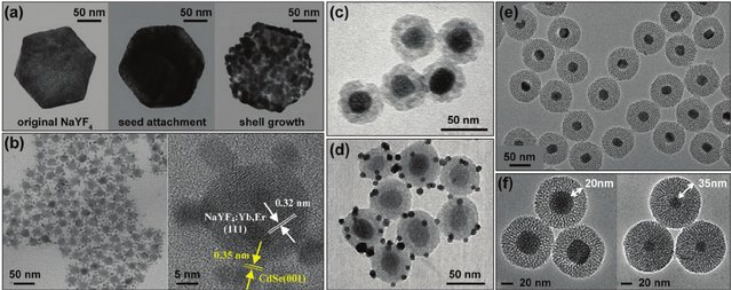
\includegraphics[width=\textwidth, height=4cm, keepaspectratio]{core.png}
                \caption{\tiny NPs core-shell no epitaxiales: (a) NaYF$_4$:Yb/Tm@Au, (b) NaYF$_4$:Yb/Er@CdSe, (c) QDs en sílice sobre NaYF$_4$:Yb/Er, (d) NPs de oro acopladas a NaYF$_4$:Yb/Er mediante sílice \cite{chen2014photon}.}
            \end{figure}
        \end{column}
    \end{columns}
\end{frame}

\begin{frame}{Resumen de la Técnica}
    \begin{alertblock}{Ventajas}
        Resolución atómica, información combinada (morfológica y cristalográfica) en un solo equipo.
    \end{alertblock}
    
    \begin{alertblock}{Desafíos}
        Alta exigencia en la preparación de la muestra (debe ser transparente a los electrones) y riesgo de dañar la muestra por la alta energía del haz.
    \end{alertblock}
\end{frame}

\begin{frame}[allowframebreaks]{Referencias}
  \printbibliography
  \nocite{*}
\end{frame}

\begin{frame}[plain]
  \centering
  \vspace{1cm}
  {\Huge Gracias.}\\[1cm]
\end{frame}

\end{document}
